\documentclass[10pt,final,leqno]{beamer}

%\usetheme{CambridgeUS}
\usetheme[style=ntnu,language=en]{ntnu2015}
%\usecolortheme{orchid}

\usepackage[utf8]{inputenc}
\usepackage[T1]{fontenc}

% Paths
\newcommand{\figs}{../figs}
\newcommand{\data}{../data}
\newcommand{\code}{../code}

% URL styles
\usepackage{url}
\urlstyle{sf}

% Units
\usepackage[detect-weight=true, binary-units=true]{siunitx}
\DeclareSIUnit\flop{FLOPS}

% Math
\usepackage{amsmath}
\usepackage{amssymb}
\usepackage{bm}
\usepackage{nicefrac}
\newcommand{\dif}[1]{{\;\text{d}#1}}

% Graphics
\usepackage{graphicx}
\usepackage{caption}
%\usepackage{subcaption}
\graphicspath{{../figs/}}

% Tikz
\usepackage{tikz}
\usetikzlibrary{positioning,shapes,arrows,calc,intersections}
\usepackage{pgfplots}
\usepgfplotslibrary{dateplot}
\pgfplotsset{compat=1.14} 

% Colors
\definecolor{darkblue}{HTML}{00688B}
\definecolor{darkgreen}{HTML}{6E8B3D}
\definecolor{cadet}{HTML}{DAE1FF}
\definecolor{salmon}{HTML}{FFB08A}

\usepackage{algorithm}

% Listings
\usepackage{textcomp}
\usepackage{listings}
\lstset{
  keywordstyle=\bfseries\color{orange},
  stringstyle=\color{darkblue!80},
  commentstyle=\color{darkblue!80},
  showstringspaces=false,
  basicstyle=\ttfamily,
  upquote=true,
}
\lstdefinestyle{fortran}{
  language=Fortran,
  morekeywords={for},
  deletekeywords={status},
}
\lstdefinestyle{c}{
  language=C,
  morekeywords={include},
}
\lstdefinestyle{glsl}{
  language=C,
  morekeywords={attribute, vec2, vec3, vec4, varying, uniform, mat2, mat3, mat4},
}
\lstdefinestyle{cuda}{
  language=C,
  morekeywords={__global__, __device__, __host__, __shared__},
}
\lstdefinestyle{shell}{
  language=bash,
  morekeywords={mkdir, ssh, cmake},
}

% Double hlines
\usepackage{hhline}

% Misc
\usepackage{nth}

\subtitle{TMA4280---Introduction to Supercomputing}

\graphicspath {{../figs/}}

\AtBeginSection[]
{
 \begin{frame}<beamer>
 \frametitle{Outline}
 \tableofcontents[currentsection]
 \end{frame}
}

\begin{document}


\title{Shared memory programming model -- OpenMP}
\institute{NTNU, IMF}
\date{February 16. 2018}
%\author{Aurélien Larcher}

\maketitle

%------------------------------------------------------------------------------
\begin{frame}
  \frametitle{Recap: Distributed memory programming model}

\textit{Parallelism with MPI}.\\
An MPI execution is started on a set of processes $\mathcal{P}$ with:
\begin{center}
\texttt{mpirun -n $N_P$ ./exe}
\end{center}
with $\texttt{$N_P$} = card(\mathcal{P})$ the number of processes.

\bigskip
A program is executed in parallel on each process:
\begin{center}
    \scalebox{0.8}{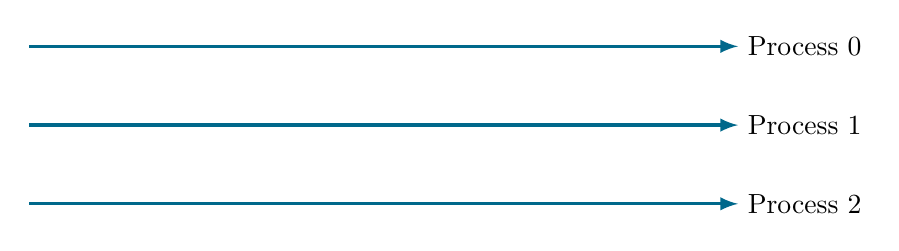
\begin{tikzpicture}
  \foreach \i in {0,...,2} {
    \draw[darkblue, very thick, -latex] (0,-\i) -- (9,-\i);
    \node[anchor=west] at (9,-\i) {Process \i};
  }
\end{tikzpicture}
}
\end{center}
where each process in $\mathcal{P} = \lbrace P0, P1, P2 \rbrace$ has a access to data in its memory space: remote data exchanged through interconnect.

\medskip
An ordered set of processes defines a \textbf{Group} (\texttt{MPI\_Group}): the inital group (\texttt{WORLD}) consists of \textbf{all} processes.

\end{frame}

%------------------------------------------------------------------------------
\begin{frame}
\frametitle{Recap: Distributed memory programming model}

Two motivations for leveraging another type of parallelism:\\[2ex]
\begin{enumerate}
\item Parallelization with MPI requires substantial changes:
\begin{itemize}
\item explicit programming
\item using an external library
\item adding functions to exchange data, perform collective operations
\end{itemize}

The programmer needs to define data structures to divide work then handle data communication: it may alter heavily his serial implementation, intrusive.
\bigskip
\item Single core performance has reached its limits (see ILP):
\begin{itemize}
\item Typical multiprocessor machine is now multicore,
\item NUMA architecture: a machine consists of multiple NUMA nodes (memory locality) with cache coherency,
\item Message Passing is not necessary,
\item Finer parallelism can be achieved. 
\end{itemize}

\end{enumerate}

\end{frame}

%------------------------------------------------------------------------------
\begin{frame}
\frametitle{Recap: Shared memory architecture}


\begin{figure}[h]
\caption{Example of NUMA plotted by \texttt{lstopo} utility of \texttt{hwloc}}
\scalebox{0.3}{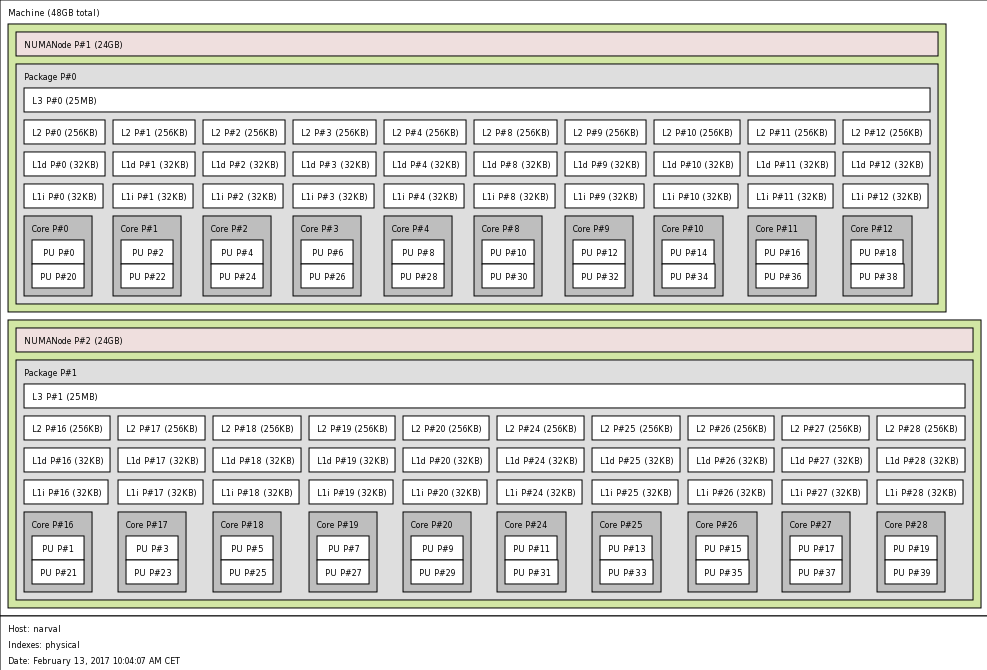
\includegraphics{\figs/narval/lstopo}}
\end{figure}

\end{frame}

%------------------------------------------------------------------------------
\begin{frame}
\frametitle{Shared memory programming model}

In a shared memory model, any worker can take a memory reference.

\medskip
Some implementations of the shared memory programming model:
\begin{itemize}
\item Native threads (UNIX System V, POSIX, Solaris, Linux)
\item Java threads (Virtual Machine)
\item OpenMP 
\item Apple Grand Central Dispatch (GCD) 
\item Intel Thread-Building Blocks (TBB)
\item \dots
\end{itemize}

\medskip
Initially developed for HPC systems and now widely used on the desktop, for example in multimedia applications.

\end{frame}

%------------------------------------------------------------------------------
\begin{frame}
\frametitle{OpenMP}

OpenMP, portable standard for shared-memory parallel programming:\\[2ex]
\begin{center}
\begin{tabular}{ll}
OpenMP 1.0 & Fortran (1997) C/C++ (1998)\\
OpenMP 1.1 & Fortran (1999)\\
OpenMP 2.5 & Fortran/C/C++ (2005)\\
OpenMP 3.0 & Fortran/C/C++ (2008)\\
OpenMP 3.1 & Fortran/C/C++ (2011)\\
OpenMP 4.0 & Fortran/C/C++ (2013)\\
OpenMP 4.5 & Fortran/C/C++ (2015)\\
\end{tabular}
\end{center}

Latest specifications introduce support \textit{offloading} to a SIMD unit, see:
\begin{center}
\url{http://www.openmp.org/specifications/}
\end{center}


\end{frame}


%------------------------------------------------------------------------------
\begin{frame}
\frametitle{OpenMP}

\begin{enumerate}
\item Thread-based parallelism
\begin{itemize}
  \item  Parallelism through concurrent use of threads
  \item  Thread of execution: minimum unit of processing which can be scheduled on a system
  \item  Thread exist with the resource of a process
  \item  Number of executing threads is defined by the user or the application
\end{itemize}
\bigskip
\item Explicit parallelism:
\begin{itemize}
  \item  Explicit, non-automatic programming model offering full control on parallelism
  \item  Does not require an external library but compiler support
  \item  Expressivity through compiler directives but also more complexe program structures through a runtime.
\end{itemize}
\end{enumerate}

\end{frame}

%------------------------------------------------------------------------------
\begin{frame}
  \frametitle{OpenMP: Program flow}
  \begin{center}
    \scalebox{0.8}{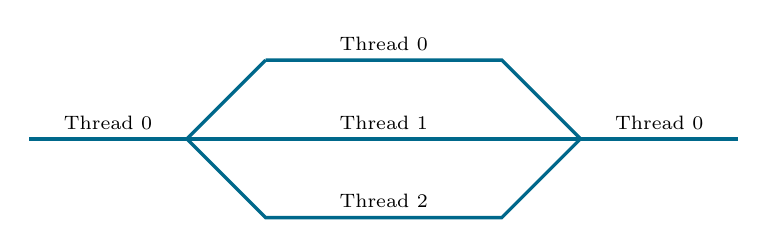
\begin{tikzpicture}
  \draw[darkblue, very thick] (0,0) -- (9,0);
  \draw[darkblue, very thick] (3,1) -- (6,1) -- (7,0) -- (6,-1) -- (3,-1) -- (2,0) -- (3,1);
  \node[anchor=south] at (8,0) {\scriptsize Thread 0};
  \node[anchor=south] at (1,0) {\scriptsize Thread 0};
  \node[anchor=south] at (4.5,1) {\scriptsize Thread 0};
  \node[anchor=south] at (4.5,0) {\scriptsize Thread 1};
  \node[anchor=south] at (4.5,-1) {\scriptsize Thread 2};
\end{tikzpicture}
}
  \end{center}
Fork/Join model:
  \begin{itemize}
  \item The main program flow happens on one processor.
  \item One master thread executes sequentially until a parallel section is encountered.
  \item \textcolor{blue}{Fork}: master thread creates a \textbf{team} of parallel threads executing the task enclosed in the parallel section.
  \item \textcolor{blue}{Parallel execution:} each thread contributes to processing,
  \item \textcolor{blue}{Join:} when the parallel section completes, spawned threads synchronize and terminate: only the master threads remains.
  \item No explicit data division is performed.
  \end{itemize}
\end{frame}

%------------------------------------------------------------------------------
\begin{frame}
\frametitle{Comparison MPI vs. OpenMP}


\begin{minipage}{0.45\textwidth}
\begin{center}
    \scalebox{0.4}{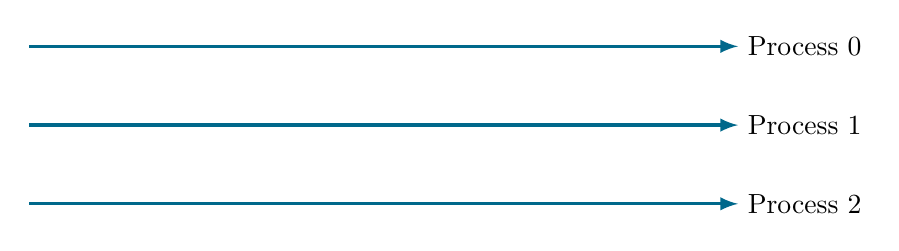
\begin{tikzpicture}
  \foreach \i in {0,...,2} {
    \draw[darkblue, very thick, -latex] (0,-\i) -- (9,-\i);
    \node[anchor=west] at (9,-\i) {Process \i};
  }
\end{tikzpicture}
}
\end{center}
\end{minipage}
\begin{minipage}{0.5\textwidth}
  \begin{center}
    \scalebox{0.5}{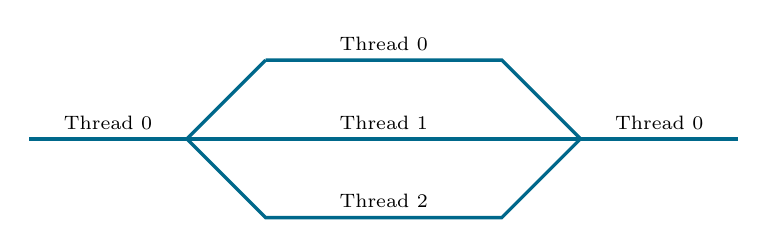
\begin{tikzpicture}
  \draw[darkblue, very thick] (0,0) -- (9,0);
  \draw[darkblue, very thick] (3,1) -- (6,1) -- (7,0) -- (6,-1) -- (3,-1) -- (2,0) -- (3,1);
  \node[anchor=south] at (8,0) {\scriptsize Thread 0};
  \node[anchor=south] at (1,0) {\scriptsize Thread 0};
  \node[anchor=south] at (4.5,1) {\scriptsize Thread 0};
  \node[anchor=south] at (4.5,0) {\scriptsize Thread 1};
  \node[anchor=south] at (4.5,-1) {\scriptsize Thread 2};
\end{tikzpicture}
}
  \end{center}
\end{minipage}

\bigskip
\begin{enumerate}
\item Parallel execution of programs\\
      vs. Concurrent execution of threads from a single execution thread.\\[2ex]
\item Each MPI process as \textit{private data} in its address space\\
      vs. All OpenMP threads may share data.
\end{enumerate}

\bigskip
\textcolor{red}{Pitfalls}: reading/writing the same memory location concurrently\\
$\rightarrow$ separate working buffers, control of resource access.

\end{frame}

%------------------------------------------------------------------------------
\begin{frame}
\frametitle{OpenMP characteristics}

\begin{itemize}
\item \textbf{Expressivity.}\\
Compiler-based directives \#pragma processed by the compiler and embedded in the source code

\medskip
\item \textbf{Nested parallelism.}\\
Placing parallel regions within parallel sections

\medskip
\item \textbf{Dynamic Threads.}\\
Runtime may change the number of threads needed to parallel sections

\medskip
\item \textbf{I/O}\\
OpenMP does not provide such specification

\medskip
\item \textbf{Memory management.}\\
A model of \textit{relaxed consistency}: threads can cache the data and not enforce consistency with main memory.
\end{itemize}

\end{frame}

\begin{frame}
  \frametitle{Operations suitable for OpenMP}
  \begin{itemize}
  \item Moderately large computation intensive operations. Since
    thread-dispatchment always has some costs attached, spawning multiple
    threads easily costs more time than what you gain by doing the calculations
    in parallel if the operations are too small.
  \item Decoupled problems. Since the threads are sharing resources, we have to
    protect resources using mutual exclusion locks if several threads need to
    read/write to the same resources concurrently. This adds code complexity and
    in most cases severe loss of performance. OpenMP shines when you are able to
    decouple problems in large, independent chunks.
  \end{itemize}
\end{frame}

%------------------------------------------------------------------------------
\begin{frame}
\frametitle{OpenMP implementations}

Compilers provide support for OpenMP:\\[2ex]
\begin{center}
\begin{tabular}{l|rrrrr}
OpenMP         & 2.5  & 3.0   & 3.1  &  4.0 & 4.5 \\
\hline\hline
GCC            & 4.2  & 4.7   & 4.7  &  4.9 & 6.1 \\
Intel          &      & 11 .0 & 12.1 & 16.0 &     \\
Clang          &      &       & 3.7  &      &     \\
Solaris Studio &      & 12.1  & 12.3 & 12.4 &     \\    
\end{tabular}
\end{center}

\medskip
Source code generation translator exists: ROSE (compiler framework) Lawrence Livermore

\medskip
Auto-parallelization can be provided by the compiler to distribute loops independently of OpenMP directives (\texttt{-xautopar} in Solaris Studio, \texttt{-ftree-parallelize-loops} in GCC), \textcolor{red}{do not mix them!}

\end{frame}

%------------------------------------------------------------------------------
\begin{frame}[fragile]
\frametitle{OpenMP implementations}

The specification defines:

\begin{enumerate}
\item Compiler Directives.
\medskip
\item Runtime Library Routines.
\medskip
\item Environment Variables.
\end{enumerate}

OpenMP ``hello world''.
\begin{lstlisting}[style=c]
  #include <omp.h>

  #pragma omp parallel
  {
    int thread = omp_get_thread_num();
    printf("Hello world from thread number %d\n",
           thread);
  }
\end{lstlisting}
The code inside the block is executed by each participating thread.

\end{frame}

%------------------------------------------------------------------------------
\begin{frame}
\frametitle{Compiler Directives}

Processed if flag passed to the compiler, and ignored otherwise.

\begin{center}
\texttt{sentinel directive-name [clause,\dots]}
\end{center}

\medskip
Applies to the next structured block of code or OpenMP construct to:
\begin{itemize}
\item Create a parallel section
\item Distribute loops across threads
\item Divide blocks of code between threads
\item Serialize a section of code
\item Synchronize the work
\item Offload data to a SIMD device (OpenMP 4.5)
\end{itemize}

\end{frame}

%------------------------------------------------------------------------------
\begin{frame}
\frametitle{Runtime Library Routines}

Compilation requires including a header and linking to a runtime library:

\begin{center}
\texttt{\#include $<$omp.h$>$}
\end{center}

\medskip
Set of functions for use in the code to:
\begin{itemize}
\item Set or query the number of threads
\item Query thread attributes
\item Set or query dynamic thread features 
\item Query if the section if parallel and the level
\item Set or query nested parallelism
\item Set, initialize or terminate locks
\item Query wall-time and resolution
\end{itemize}

\end{frame}

%------------------------------------------------------------------------------
\begin{frame}
\frametitle{Environment Variables}

\begin{center}
\texttt{OMP\_NUM\_THREADS=4 ./exe}
\end{center}

\medskip
Specified at execution to:
\begin{itemize}
\item Set the number of threads
\item Specify how loop iterations are divided
\item Bind threads to processors
\item Enable or disable nested parallelism, set nesting level
\item Set thread stack size
\item Set thread wait policy
\end{itemize}

\end{frame}

%------------------------------------------------------------------------------
\begin{frame}
\frametitle{Directive and clauses}

Each directive can be followed by clauses pertaining to its category:

\begin{itemize}
\item Parallel construct: \texttt{parallel}

\medskip
\item Work-sharing construct: \texttt{for}, \texttt{sections}, \texttt{single}

\medskip
\item Parallel Work-sharing construct: \texttt{parallel for}, \texttt{task} (OpenMP 3.0)

\medskip
\item Coordination and Synchronization: \texttt{master}, \texttt{critical}, \texttt{barrier}, \texttt{taskwait}, \texttt{atomic}, \texttt{flush}, \texttt{ordered}, \texttt{threadprivate}

\end{itemize}

\medskip
Clauses can be categorized as well:
\begin{enumerate}
\item Data sharing clauses
\item Data copying clauses
\item Map clauses (OpenMP 4.0)
\item SIMD clauses (OpenMP 4.0)
\end{enumerate}

\end{frame}

%------------------------------------------------------------------------------

\begin{frame}[fragile]
  \frametitle{Loop distribution: fixed cost}

Loop distribution is an instance of Data Parallelism.\\
$\rightarrow$ scalability w.r.t the data.

\bigskip

  \begin{lstlisting}[style=c]
    for (int i = 0; i < 100; i++)
      do_something(i);
  \end{lstlisting}
  \begin{itemize}
  \item We assume that \texttt{do\_something} does not depend on any global
    resources: each call is independent of any other call.
  \item To split this loop among several threads, you can simply do
    \begin{lstlisting}[style=c]
#pragma omp parallel for schedule(static)
for (int i = 0; i < 100; i++)
  do_something(i);
    \end{lstlisting}
  \end{itemize}
\end{frame}

\begin{frame}[fragile]
  \frametitle{Loop distribution: fixed cost}
  \begin{lstlisting}[style=c]
    #pragma omp parallel for schedule(static)
  \end{lstlisting}
  The pragma has three parts:
  \begin{itemize}
  \item \texttt{\#pragma omp}: all OpenMP directives start with this.
  \item \texttt{parallel for}: tells the compiler that the following for-loop
    should be parallelized.
  \item \texttt{schedule(static)}: tells the compiler to give each thread
    approximately the same number of iterations up-front.
  \end{itemize}
\end{frame}

\begin{frame}[fragile]
  \frametitle{Loop distribution: varying cost}
  If each call to \texttt{do\_something(i)} takes a different amount of time,
  depending perhaps on \texttt{i}, we can use dynamic scheduling:
  \begin{lstlisting}[style=c]
    #pragma omp parallel for schedule(dynamic)
    for (int i = 0; i < 100; i++)
      do_something(i);
  \end{lstlisting}
  This instructs the compiler not to divide the work up-front, but instead leave
  one thread as a ``broker''. Initially, each thread is assigned a single
  iteration. Upon completing this, they ask the broker for more work. The broker
  keeps handing out work until each iteration has been assigned.
\end{frame}

\begin{frame}[fragile]
  \frametitle{Loop distribution: varying cost}
  \begin{itemize}
  \item This works well if there are many iterations, and each of them are
    suitably expensive.
  \item If the iterations are cheap, then execution time will be dominated by
    negotiating with the broker thread, since this can only happen serially.
  \item We can minimize this problem by specifying a \emph{chunk size},
  \begin{lstlisting}[style=c]
#pragma omp parallel for schedule(dynamic, 5)
for (int i = 0; i < 100; i++)
  do_something(i);
  \end{lstlisting}
  \item Now, the broker hands out assignments in chunks of five. Each chunk is
    now expensive enough that the broker is not overrun.
  \end{itemize}
\end{frame}

\begin{frame}[fragile]
  \frametitle{Loop distribution: varying cost}
  \begin{itemize}
  \item By using a fixed chunk size, we may end up in a situation where all the
    remaining work is assigned to a single thread. (Poor load balancing.)
  \item OpenMP offers a third scheduling mode to help fix this problem.
  \begin{lstlisting}[style=c]
#pragma omp parallel for schedule(guided, 5)
for (int i = 0; i < 100; i++)
  do_something(i);
  \end{lstlisting}
  \end{itemize}
\end{frame}

%------------------------------------------------------------------------------

\begin{frame}
\frametitle{Loop distribution: scheduling policies}

Scheduling policies aim at devising an optimal division of work.

\bigskip

Several policies are available in OpenMP:\\[2ex]
\begin{tabular}{l|l}
\textbf{Name}  & \textbf{Policy}\\
\hline\hline
\texttt{static} & \textit{a priori} division of work based on loop\\
\texttt{dynamic} & load-balancing of work during runtime by one thread\\
\texttt{dynamic, N} & same as dynamic but with hint about data chunk size\\
\texttt{guided, N} & same as previous but with decrease of chunk size policy\\
\texttt{auto, N} & automatically determined at runtime\\
\texttt{runtime, N} & specified at runtime by environment variable\\
\end{tabular}

\bigskip
Chosing one of them depends on the nature of the work (fixed or varying cost) and the granularity of the work (minimum amount of work as compared to overhead).

\end{frame}

%------------------------------------------------------------------------------
\begin{frame}[fragile]
  \frametitle{Task distribution: sections}

Task distribution is an instance of Task/Function Parallelism.\\
$\rightarrow$ scalability w.r.t logical division into subtasks.

\bigskip
  Consider the serial snippet
  \begin{lstlisting}[style=c]
    do_job_1();
    do_job_2();
    do_job_3();
  \end{lstlisting}
  Again we assume that the jobs are independent and share no resources, but they
  are different enough in nature that it doesn't make sense to write this in the
  form of a loop.
\end{frame}

\begin{frame}[fragile]
  \frametitle{Task distribution: sections}
  This can be parallelized as such.
  \begin{lstlisting}[style=c, basicstyle=\ttfamily\footnotesize]
    #pragma omp parallel sections
    {
      #pragma omp parallel section
      {
        do_job_1();
      }
      #pragma omp parallel section
      {
        do_job_2();
      }
      #pragma omp parallel section
      {
        do_job_3();
      }
    }
  \end{lstlisting}
\end{frame}

\begin{frame}[fragile]
  \frametitle{Shared and private variables}
  As a rule,
  \begin{itemize}
  \item variables that are declared \emph{outside} the parallel construct are
    shared between threads. Extra care must be taken when writing to these
    variables, and it should preferably be avoided if at all possible.
  \item variables that are declared \emph{inside} are private: each thread has
    its own copy of it. Since a parallel block defines a scope, these variables
    do not leak out to the surrounding serial scope.
  \end{itemize}
  It is possible to override this using \texttt{private(...)} and
  \texttt{shared(...)} directives in OpenMP pragmas, where in each case the
  \ldots is a list of variables.
\end{frame}

\begin{frame}[fragile]
  \frametitle{Example: summing a vector}
\begin{lstlisting}[style=c]
  double vec[N] = { ... };
  double sum = 0.0;

  #pragma omp parallel for
  for (size_t i = 0; i < N; i++)
    sum += vec[i];
\end{lstlisting}
  Here, \texttt{i} is private and \texttt{sum}, \texttt{vec} and \texttt{N} are
  shared. \\~\\

  We are writing to a shared variable. How do we solve this?
\end{frame}

\begin{frame}[fragile]
  \frametitle{Example: summing a vector}
  OpenMP supports the \emph{reduction} directive for precisely this kind of
  situation.
\begin{lstlisting}[style=c]
  double vec[N] = { ... };
  double sum = 0.0;

  #pragma omp parallel for reduction(+:sum)
  for (size_t i = 0; i < N; i++)
    sum += vec[i];
\end{lstlisting}
  Now, each thread gets its private variable \texttt{sum}, and after the loop,
  each of these variables are summed into the shared one.
\end{frame}

%------------------------------------------------------------------------------
\begin{frame}
\frametitle{Critical sections}

Case: several threads need access to the same resource.
$\rightarrow$ allow access to one thread \textbf{only}: resource locking.

\medskip
\textit{Critical section} is a program section which can only be executed by one thread at any time.

\medskip
Managing unique acces to a resource can be achieved by a \textit{mutual exclusion} mechanism, also called \textit{mutex}.

\end{frame}

%------------------------------------------------------------------------------
\begin{frame}[fragile]
  \frametitle{Critical sections}
  \begin{center}
    \scalebox{0.8}{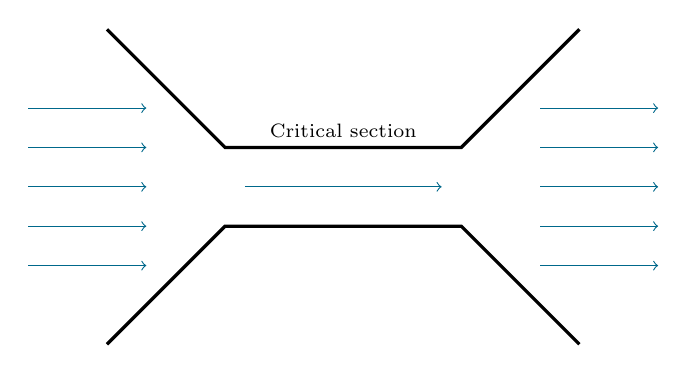
\begin{tikzpicture}[scale=0.5]
  \draw[very thick] (-6,4) -- (-3,1) -- (3,1) -- (6,4);
  \draw[very thick] (-6,-4) -- (-3,-1) -- (3,-1) -- (6,-4);
  \draw[darkblue, ->] (-2.5,0) -- (2.5,0);
  \foreach \i in {-2,...,2} {
    \draw[darkblue, ->] (-8,\i) -- (-5,\i);
    \draw[darkblue, ->] (5,\i) -- (8,\i);
  }
  \node[anchor=south] at (0,1) {\scriptsize Critical section};
\end{tikzpicture}
}
  \end{center}
  A critical section is a part of the code that, for whatever reason, should
  only be accessed by one thread at a time. Typically this happens whenever you
  need to read or write from or to shared resources.
\end{frame}

\begin{frame}[fragile]
  \frametitle{Critical sections: explicit locks}
  You can use mutexes (\emph{mutual exclusion locks}) for this.
  \begin{lstlisting}[style=c]
    omp_lock_t my_lock;
    omp_init_lock(&my_lock);

    #pragma omp parallel for
    for (int i = 0; i < 100; i++) {
      do_something(i);

      omp_set_lock(&my_lock);
      // critical section
      omp_unset_lock(&my_lock);
    }

    omp_destroy_lock(&my_lock);
  \end{lstlisting}
\end{frame}

\begin{frame}[fragile]
  \frametitle{Critical sections: pragmas}
  OpenMP has built-in language support for critical sections.
  \begin{lstlisting}[style=c]
    #pragma omp parallel for
    for (int i = 0; i < 100; i++) {
      do_something(i);

      #pragma omp critical
      {
        // critical section
      }
    }
  \end{lstlisting}
\end{frame}

\begin{frame}[fragile]
  \frametitle{Critical sections: pragmas}
  You can even have named critical sections.
  \begin{lstlisting}[style=c, basicstyle=\ttfamily\footnotesize]
    #pragma omp parallel for
    for (int i = 0; i < 100; i++) {
      do_something(i);

      #pragma omp critical updateLog
      {
        // update the log file
      }

      do_something_else(i);

      #pragma omp critical updateLog
      {
        // update the log file
      }
    }
  \end{lstlisting}

\textcolor{red}{Pitfall}: A critical section suffers then from \textit{serialization}.\\
$\rightarrow$ Crucial for efficiency, remember Amdahl's law!
\end{frame}

\begin{frame}[fragile]
  \frametitle{How to enable}
  \begin{itemize}
  \item With GNU compilers (\texttt{gcc}, \texttt{g++}, \texttt{gfortran}), use
    the compiler flag \texttt{-fopenmp}.
  \item With Intel compilers (\texttt{icc}, \texttt{icpc}, \texttt{ifort}), use
    the compiler flag \texttt{-openmp}.
  \item Without this flag, GNU compilers will silently ignore pragmas, while
    Intel compilers will give a warning. In either case, the resulting binary is
    equivalent to serial code.
  \item In CMake you can do this
    \begin{lstlisting}[basicstyle=\ttfamily\footnotesize]
find_package(OpenMP)
if(OPENMP_FOUND)
  set(CMAKE_C_FLAGS
      "${CMAKE_C_FLAGS} ${OpenMP_C_FLAGS}$")
endif()
    \end{lstlisting}
%$
  \end{itemize}
\end{frame}

\begin{frame}[fragile]
  \frametitle{Number of threads}
  The number of threads spawned is determined in the following order.
  \begin{enumerate}
  \item Programs can call \texttt{omp\_set\_num\_threads(int)} to request a number
    of threads at runtime. This function is defined in \texttt{omp.h}.
  \item The environment variable \texttt{OMP\_NUM\_THREADS}, if it exists. You can
    run your programs in most shells as
    \texttt{OMP\_NUM\_THREADS=8 ./myprogram}.
  \item A sensible default value which depends on your system hardware and the data.
    Typically this will be the number of logical cores.
  \end{enumerate}
\end{frame}

\begin{frame}
  \frametitle{Conclusions}
  \begin{itemize}
  \item OpenMP offers easy exploitation of computing resources on shared memory
    machines.
  \item The parallel code is very close to the serial code - it usually only
    differs by some pragmas which you can tell a compiler to ignore.
  \item The fork-join programming model often is harder to grasp than the
    distributed model, in particular if several threads need to access the same
    resources.
  \item Best results are usually achieved if you combine OpenMP and MPI. This is
    also the model that maps the best to modern hardware, where you typically
    have a few handfuls of CPUs sharing memory, while using more than that
    requires a distributed memory programming model.
  \end{itemize}

Example code: using OpenMP for the parallel assembly of the linear system in a C++ finite element code. Notice that \texttt{for} loops should be made explicit!
\end{frame}

\begin{frame}
  \frametitle{More information}
  \begin{center}
    The official page for the OpenMP specification can be found at \\~\\
    http://openmp.org including very helpful summary documents!\\~\\~\\~\\
    Some very instructive tutorials can be found at \\~\\
    http://computing.llnl.gov/tutorials/openMP
  \end{center}
\end{frame}

%------------------------------------------------------------------------------

\end{document}

